\chapter{Apéndice}

\section{Apéndice de soluciones en implementación}

\subsection{Si la placa deja de ser detectada}
En la primera subida del programa con los datos de entrenamiento
creados por mí, la placa dejó de ser detectada por el ordenador.\\
Lo cual me llevó a pensar que el bootloader se había corrompido.
Sin embargo, buscando posibles causas, encontré una solución:
restaurar manualmente la placa, cosa que solo funciona, evidentemente,
si el bootloader no está dañado.
Pulsando el botón reset de la placa rápidamente varias veces justo
al conectarlo al ordenador, puede restaurarse la placa. Si ha funcionado,
el "L" led se encenderá.

Esto ocurría al incorporar el modelo de datos que yo mismo entrenaba
y fue uno de los problemas que más tiempo me llevó solucionar, sobre
todo porque no tenía ningún tipo de referencia de por qué no estaba
respondiendo correctamente el programa con el nuevo modelo.\\
Por suerte llegué a la solución:\\~\\


\subsection{El modelo de datos entrenado no responde\cite{intro-tensor-micro}}
Como explico en caso anterior, la incorporar el modelo de datos
entrenado con el dataset de ejemplo que proporciona TensorFlow,
al subir el programa a la placa, esta dejaba de reconocerse por
el ordenador, teniendo que resetear la flash de la placa.\\
Esto se debía a que el proyecto Arduino no soportaba una de las
operaciones que realiza nuestro modelo(reshape).\\
\newpage Podemos solucionar esto de dos formas:
\begin{enumerate}
    \item (No probada) Simplemente hacer uso de AllOpsResolver,
    de forma que el interprete tendrá acceso a todas las operaciones
    disponibles.
    \item Esta segunda es la más sofisticada, ya que al no disponer
    de todas las operaciones para el interprete, reduciremos la cantidad
    de memoria que ocupamos.\\Es la que yo implementé.
\end{enumerate}

Añadir la siguiente línea al archivo \small\textbf{*.ino}\normalsize~
de nuestro proyecto:
\begin{lstlisting}
micro_mutable_op_resolver.AddBuiltin(tflite::BuiltinOperator_RESHAPE,
                                      tflite::ops::micro::Register_RESHAPE());
\end{lstlisting}

De esta forma estamos añadiendo la operación al repertorio de las que tendrá
disponibles el interprete\small\textit{(static\_interpreter)}\normalsize,
\small\textbf{micro\_mutable\_op\_resolver}\normalsize.

\begin{figure}[h]
\begin{lstlisting}[firstnumber=72]
static tflite::MicroMutableOpResolver micro_mutable_op_resolver;  // NOLINT
micro_mutable_op_resolver.AddBuiltin(
    tflite::BuiltinOperator_DEPTHWISE_CONV_2D,
    tflite::ops::micro::Register_DEPTHWISE_CONV_2D());
micro_mutable_op_resolver.AddBuiltin(
    tflite::BuiltinOperator_MAX_POOL_2D,
    tflite::ops::micro::Register_MAX_POOL_2D());
micro_mutable_op_resolver.AddBuiltin(tflite::BuiltinOperator_CONV_2D,
                                     tflite::ops::micro::Register_CONV_2D());
micro_mutable_op_resolver.AddBuiltin(
    tflite::BuiltinOperator_FULLY_CONNECTED,
    tflite::ops::micro::Register_FULLY_CONNECTED());
micro_mutable_op_resolver.AddBuiltin(tflite::BuiltinOperator_SOFTMAX,
                                     tflite::ops::micro::Register_SOFTMAX());
micro_mutable_op_resolver.AddBuiltin(tflite::BuiltinOperator_RESHAPE,
                                     tflite::ops::micro::Register_RESHAPE());
                                     
// Build an interpreter to run the model with
static tflite::MicroInterpreter static_interpreter(
    model, micro_mutable_op_resolver, tensor_arena, kTensorArenaSize,
    error_reporter);
interpreter = &static_interpreter;
\end{lstlisting}
\caption{Fragmento de \small\textbf{*.ino}\normalsize~ de nuestro proyecto.}
\end{figure}

Este fragmento de código ilustra lo que acabo de explicar.


\subsection{Error durante el entrenamiento}
Al comenzar con mi primer pequeño dataset para comprobar cuán realizable es
mi idea para este modelo, tuve un error que me tuvo durante un buen tiempo
ocupado.

\begin{figure}[h]
    \centering
    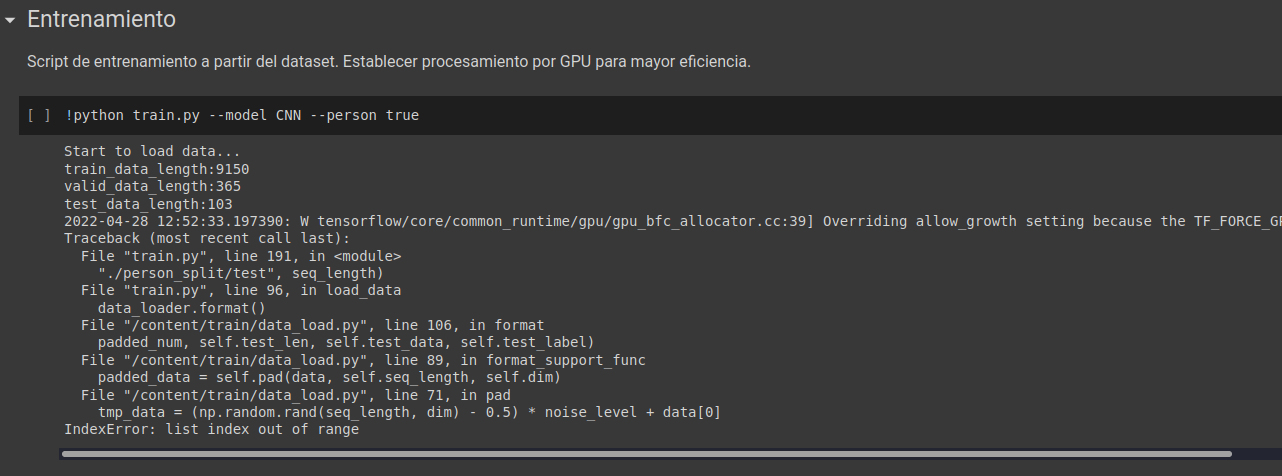
\includegraphics[width=1\textwidth]{capturas/ErrorEntrenamiento.png}\\[-0,40cm]
    \caption{Error durante primer entrenamiento con un dataset propio.}
    \end{figure}

Tras revisar que no se debía a la longitud de las secuencias de datos,
como hace pensar el mensaje de error, fui a intentar reducir el tamaño de las
muestras del dataset y fue cuando vi que había un error en una de las muestras,
de forma que había un separador (' -,-,-') sin información.\\
Al eliminarlo, el entrenamiento ya no arrojaba errores.


\subsection{Error al cambiar el tamaño de las secuencias de movimientos}
Los movimientos que se deben registrar para las letras son, en general, más complejos
que los que incluye el dataset de ejemplo. Por lo tanto las secuencias de registro
de movimiento, serán mayores. Esto supone un problema porque el modelo está ajustado
al dataset de ejemplo y por tanto, se queda algo corto para nuestro propósito.
El error se da al cambiar el tamaño de dicha secuencia
(\small\textbf{seq\_length}\normalsize) en \small\textbf{train.py}\normalsize~ y
\small\textbf{train\_test.py}\normalsize~.

\begin{figure}[h]
    \centering
    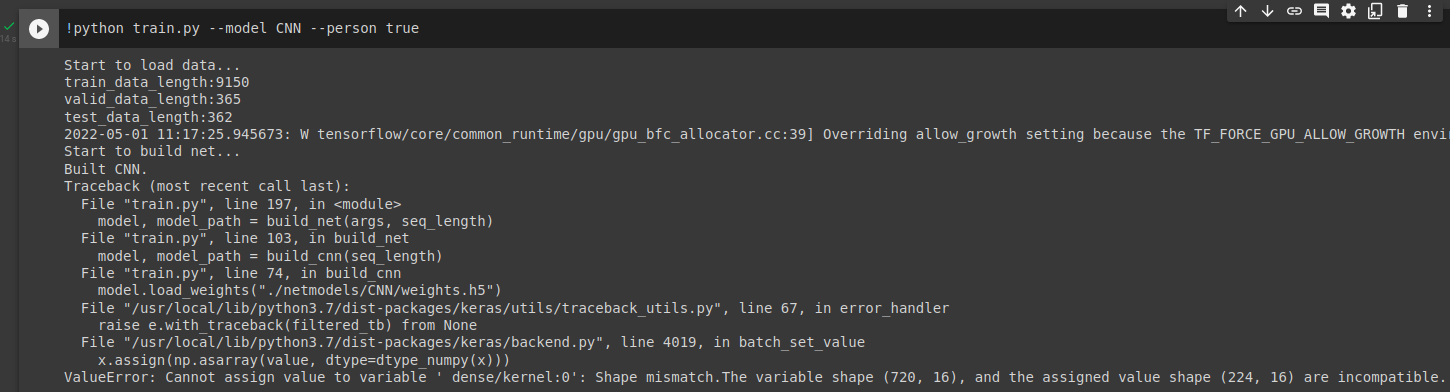
\includegraphics[width=1\textwidth]{capturas/ErrorTamanioSecuencias.png}\\[-0,40cm]
    \caption{Error al cambiar el tamaño de secuencia de movimientos.}
    \end{figure}

Tras mucha documentación sobre Tensorflow, y no obtener la causa del error; pensé
que esto ya me pasó por culpa de la configuración del \small\textbf{*.ino}\normalsize~.
Así que fui a revisarlo y efectivamente, hay un parámetro en este archivo sujeto a
la longitud de los datos. Tras cambiarlo, funcionaba correctamente de nuevo, aunque
sin detectar la letra que estaba probando en el nuevo dataset.


\subsection{Valores nulos al leer por Bluetooth QT}
Tras mucho tiempo implementando e intentando dar con el error de por qué no se
leía ninguna characteristic del dispositivo pese a estar detectándolas y estar
correctamente conectado, se debía a dos factores.\\
El primero estar haciendo uso de una librería anterior a la documentación con
la que estaba trabajando(Librería de QLowEnergyService). Hay grandes diferencias
en el comportamiento de algunos métodos de esta librería de las versiones 5.x
a la 6.x, aunque por desgracia, estas no provocan errores, hacen que el
el código no funcione como se esperaría(Enums con valores diferentes o inexistentes, etc).\\
En segundo lugar estaba llamando a un método cuando todavía no se había recibido
la characteristic. Por tanto esta aparentaba estar bien registrada, ya que
podía obtener su Uuid, pero no contenía ningún valor.
Estaba leyendo en connectToService() y no en serviceDetailsDiscovered().\\

He instalado  ArduinoBLE.h para probar sketch de harvard\\
\url{https://create.arduino.cc/projecthub/sibo_gao/harry-potter-magic-wand-384477}


Orientación para vTensorFlow no Harvard:
\url{https://github.com/andriyadi/MagicWand-TFLite-Arduino/blob/master/src/accelerometer_handler.cpp}


Para modo pizarra:
\url{https://github.com/petewarden/magic_wand/blob/main/website/index.html}.
\url{https://tinyml.seas.harvard.edu/magic_wand/}


\section{Apéndice teórico}